\documentclass{article}
\usepackage{xeCJK}
\linespread{1.1}
\setCJKmainfont{WenQuanYi Micro Hei}
\title{Extendible Hashing项目实验报告}
\author{10389048杨帆 \\ 10389084梁展瑞 \\ 12924901古宣佑}
\begin{document}
\maketitle
\section{摘要}
\section{实验环境与工具}
    \begin{enumerate}
        \item Operating system: Linux(Debian \& Arch \& Ubuntu, with 3.0+ kernels)
        \item Language: C
        \item Compiler: GCC
        \item Documentation: \LaTeX , asciidoc, Markdown
        \item Collaboration Platform/Project Hosting: GitHub
        \item Debug utils: GDB, python, perf, gprof, xdot, gprof2dot, VIM(to do regex matching often)
        \item Editor: VIM
    \end{enumerate}
    \paragraph{}
        这是在GitHub上的repo,可以看到多个branch及历史记录。
    \begin{verbatim}
https://github.com/ddmbr/Extendible-Hashing/
    \end{verbatim}
\section{流程总览}
    \paragraph{}
        整个流程可以划分为建立和查询两个大方面,分别叙述如下。(repo有初期使用的草稿:draft.txt)
    \subsection{建立数据库}
        \paragraph{}
            考虑到一个情况,当同时有大量的相同key的数据插入时,会导致一个桶无法分裂而必须拉链。但事前的统计发现,
        \begin{enumerate}
            \item key相同的条目最多只有7条。
            \item 依照我们的实现方式,每个桶的容量大概在100条。
        \end{enumerate}
        \paragraph{}
            所以我们的程序没有加入拉链的方法。以下是简要流程。
\begin{verbatim}
While the end of the raw file(i.e, lineitem.tbl) is not reached, 
    Load a page from the raw file to the memory.
    Loop through the page, to:
        Read the next record in the page.
        Get its key.
        Get the hash value `hv' of the key.
        Fetch the corresponding index page,
        According to the index, fetch the corresponding
        bucket page.
        Before inserting the record, check that 
        whether the bucket will be overflowed.
            If yes,
                If global depth == local depth,
                    Double the index
            Then split the bucket and redistribute.
        Write the record into the page.

\end{verbatim}
    \subsection{查询}
\begin{verbatim}
While not reach the end of the query,
    Read next specific key.
    Get the hash value `hv' of the key.
    Fetch the corresponding bucket
    Loop through the bucket and print the matched records.
\end{verbatim}
\section{架构}
    \subsection{总览}
        \paragraph{}
            程序大致划分为4个模块,分别为File Manager, Buffer Manager, Parser以及Hash。
        \begin{itemize}
            \item File Manager主要跟磁盘相关的操作,例如在磁盘上申请新页。
            \item Buffer Manager处理跟内存管理相关的操作,例如换页等,时钟页面算法的核心在这个模块里。
            \item Parser处理和源文本文件(lineitem.tbl)读取相关的操作。
            \item Hash模块则处理和哈希算法相关的操作,含有Extendible Hashing的核心。
        \end{itemize}
        \paragraph{}
            在数据结构上,设计了page\_t和record\_t两个重要的结构体,用于存储页(使用void*)和存储记录,附带一些必要信息,如页号,并相应有多种相关方法。比如,将record\_t转换成可以输出的字符串,在page\_t中的页面二进制数据中抓取出指定的记录并转成record\_t,等等。完整方法详见src/ehdb\_record.h,已附有详细注释。
    \subsection{关键实现说明}
        \begin{enumerate}
            \item 时钟页面算法
                \paragraph{}
                    用于进行页面置换的调度。是FIFO算法的一个改良。该算法将所有管理的页面用一个最大长度循环列表放置, 每个页面附加一个标志位R, 另外有一个“时钟指针”, 指向其中一个页面 。页面放满且有新页面调入时, 按以下步骤决定换出的页面.
                    \begin{enumerate}
                        \item 如果指针指向的页面的R位是0, 则换出这个页面;
                        \item 否则,将指针所指页面R位置0,将指针指向列表中下一个页面(注意列表是循环的)
                        \item 重复直到找到R位为0的页面。
                    \end{enumerate}
                \paragraph{}
                    对于换入的新页面,R位置1.
            \item 桶分裂/目录翻倍
                \paragraph{}
                    一个桶分裂之后,一个很重要的细节是,要把相关的那些索引正确地分指到两个桶。
                \paragraph{}
                    一个朴素的做法是,从头到尾地扫描记录,提取出与原桶相关的记录并修改。但这样效率很低,原因是换页率高。假设Local Depth为k,扫描的时候按(1 << k)的步长扫,则速度会快很多。不同做法效率如下
                \begin{itemize}
                    \item 优化前,导入lineitem.tbl全部花7分钟左右
                    \item 优化后,导入lineitem.tbl全部花4分钟左右,其中,IO在300万次左右。
                \end{itemize}
            \item 记录压缩
                \paragraph{}
                    记录的存储一个非常方便的方式是,整个当作大字串存起来,需要的时候往里面提取并分析。然而这样非常耗空间,因为把数字当作了字符串存。假设一个数字有11位,按字符串存需要11 byte,假设按int存的话,只需4 byte,压缩比例为11:4,相当客观。
                \paragraph{}
                    另外,对于日期我们单独处理,连同年月日一起当做int存储。以下是完整的格式
\begin{verbatim}
struct record_t{
    identifier_t orderkey, 
               partkey, 
               suppkey;
    int linenumber;
    decimal_t quantity,
            extendedprice,
            discount,
            tax;
    flag_t returnflag,
           linestatus;
    date_t shipdate,
           commitdate,
           receiptdate;

    char shipinstruct[25+1];
    char shipmode[10+1];
    char comment[44+1];
};
\end{verbatim}
                \paragraph{}
                    压缩存储能节省空间,这样能省下IO时间。经测试少了大概5/1的硬盘存储空间,节省了约2分钟。
        \end{enumerate}
\section{结果与分析}
    \subsection{Profile}
        \paragraph{}
            以下是不同模块耗时的分析,以便于优化。
        \paragraph{}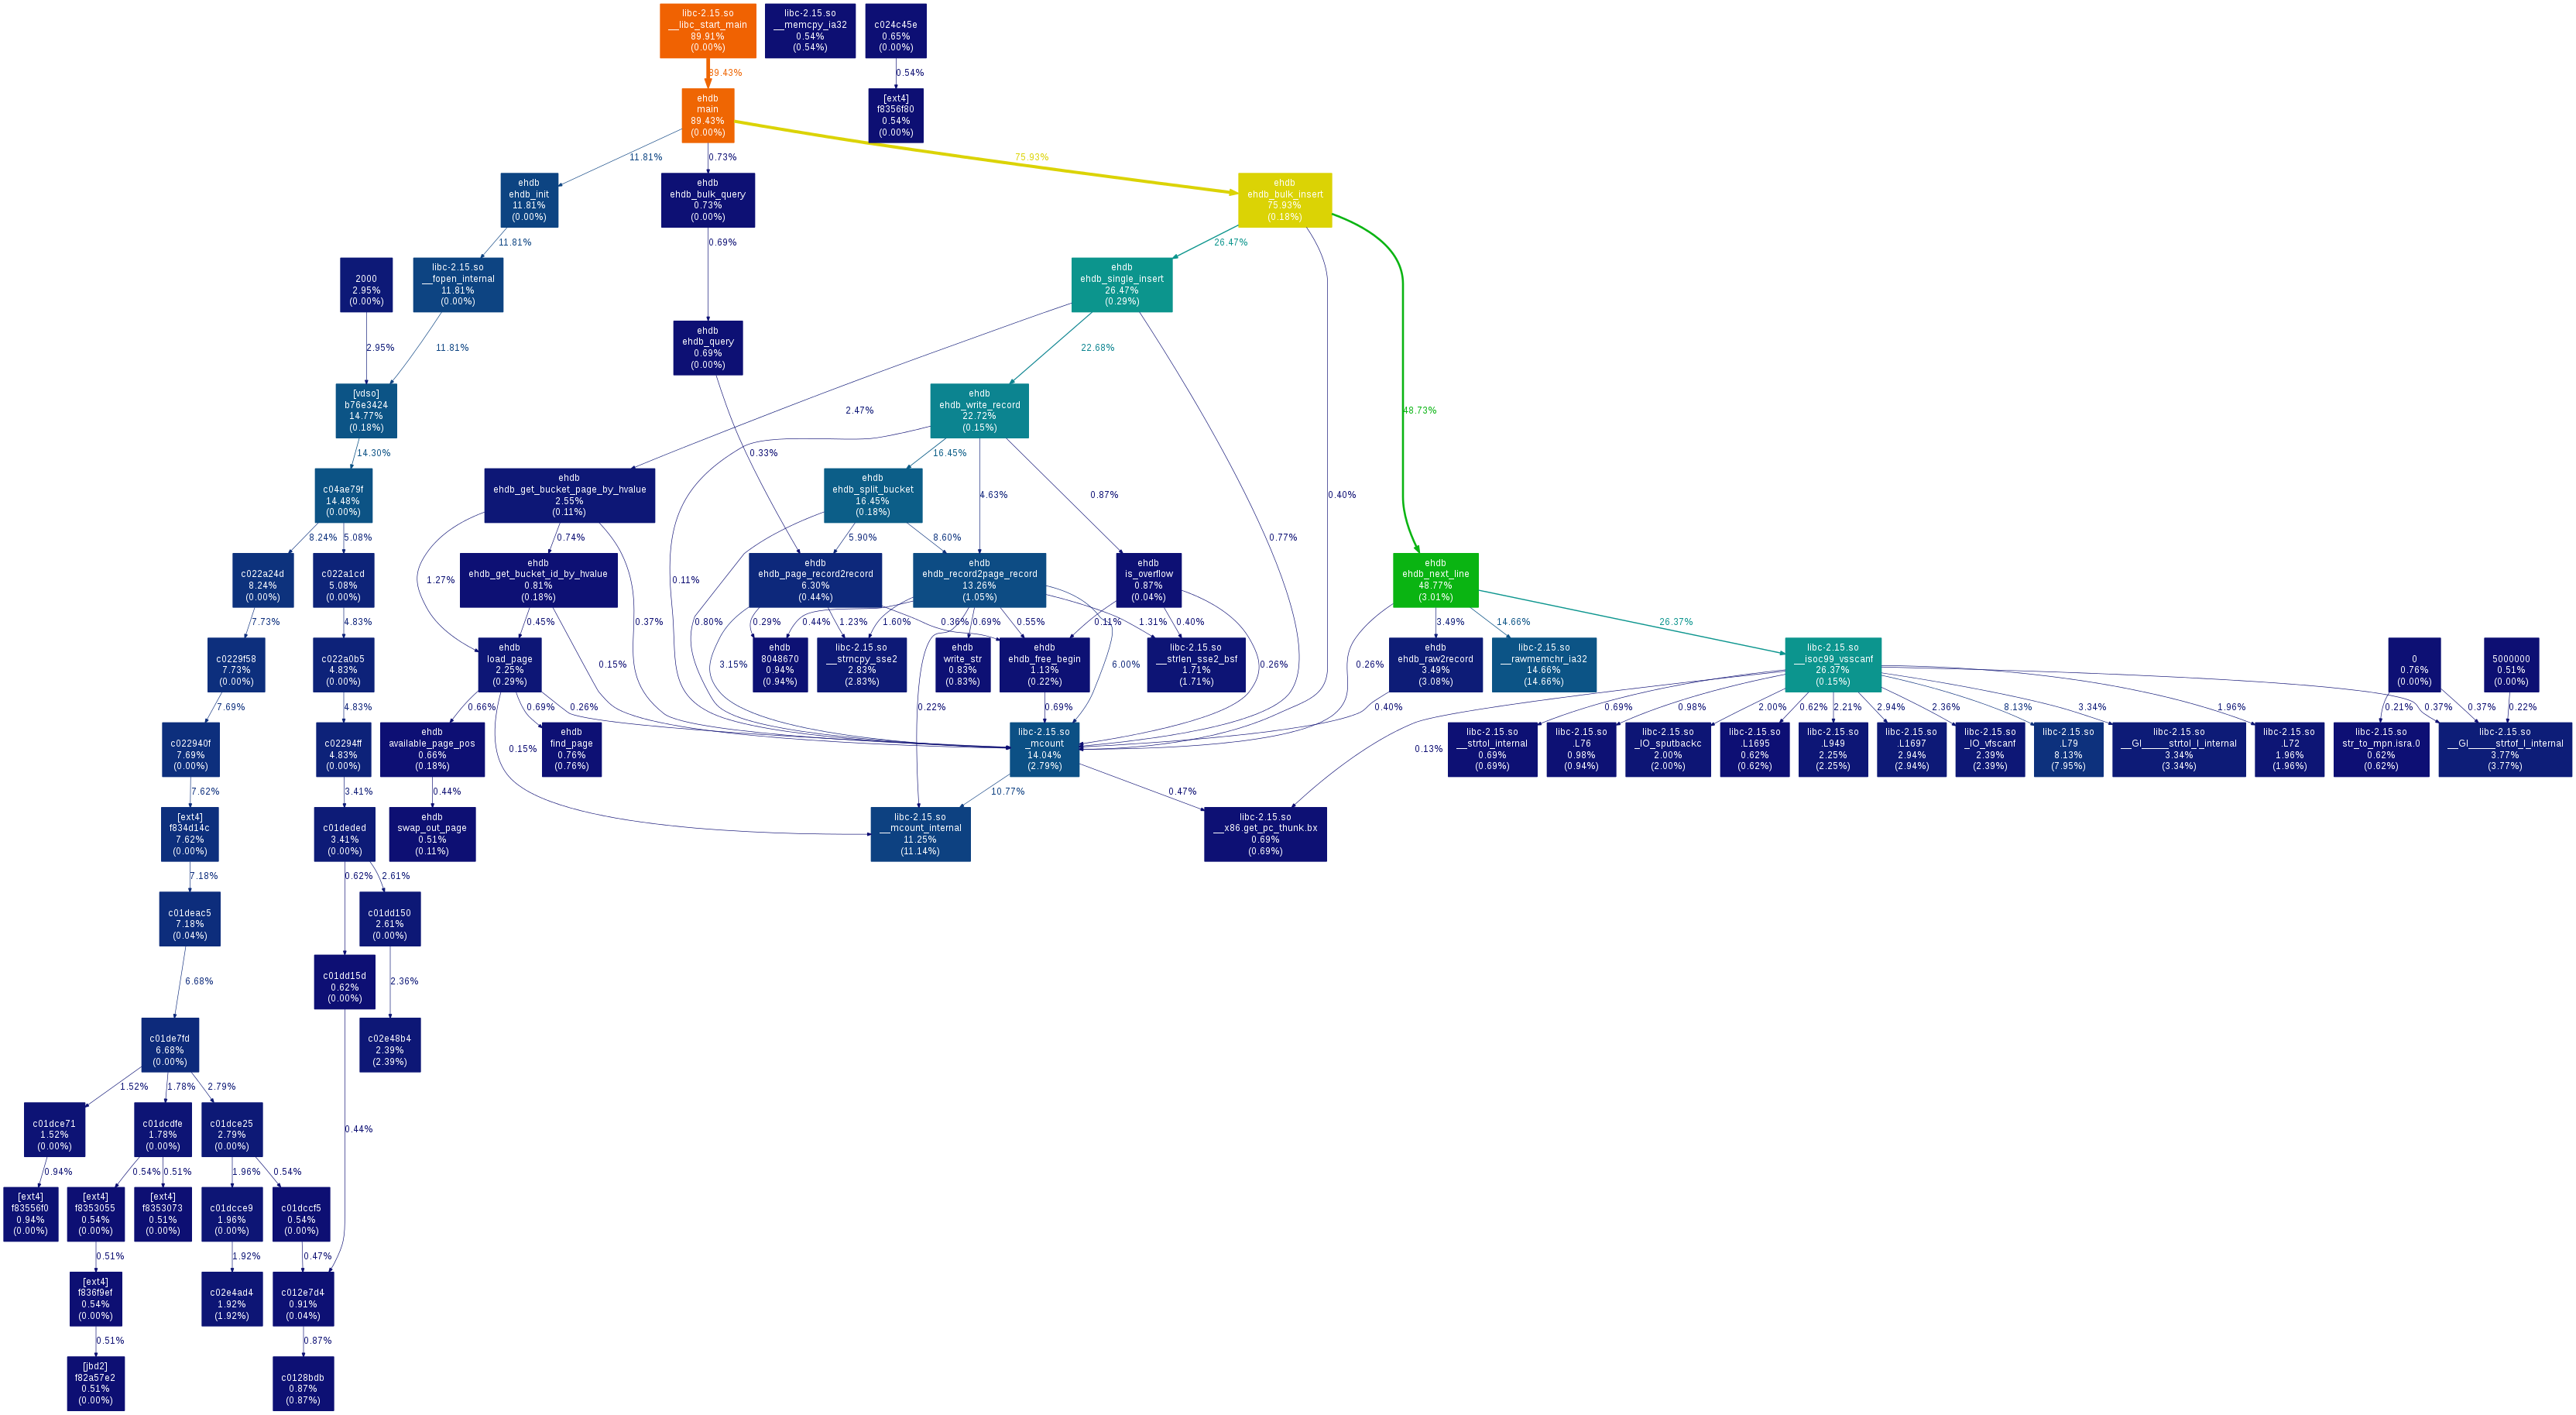
\includegraphics[scale=0.5]{proff_big_record_perf.png}
        \paragraph{}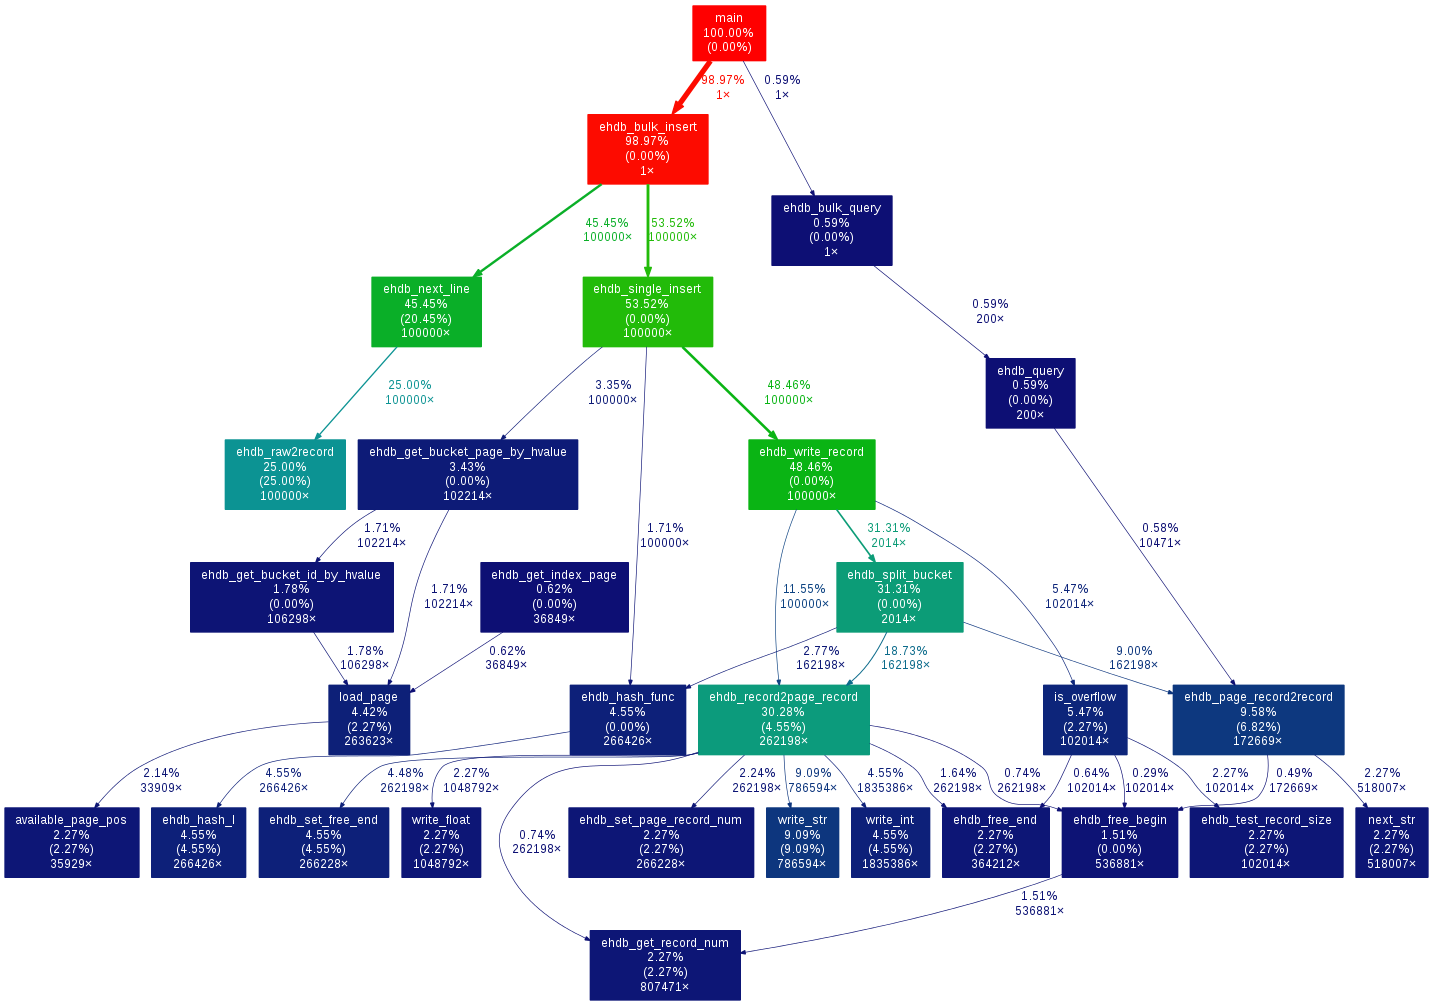
\includegraphics[scale=0.5]{proff_big_record.png}
    \subsection{记录分布情况}
        \paragraph{}
            低位哈希时,5000条记录在所有桶上的分布情况
        \paragraph{}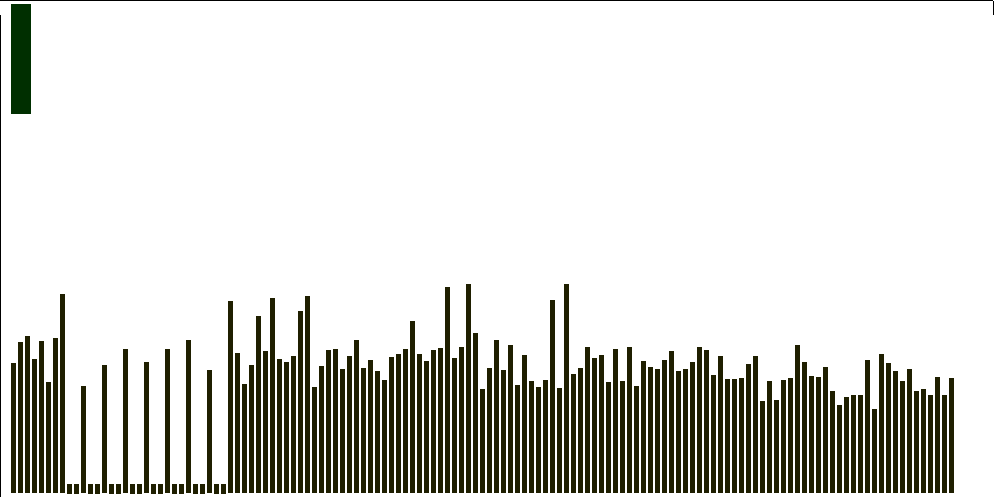
\includegraphics[scale=0.5]{pic5000_l.png}
        \paragraph{}
            高位哈希时,5000条记录在所有桶上的分布情况
        \paragraph{}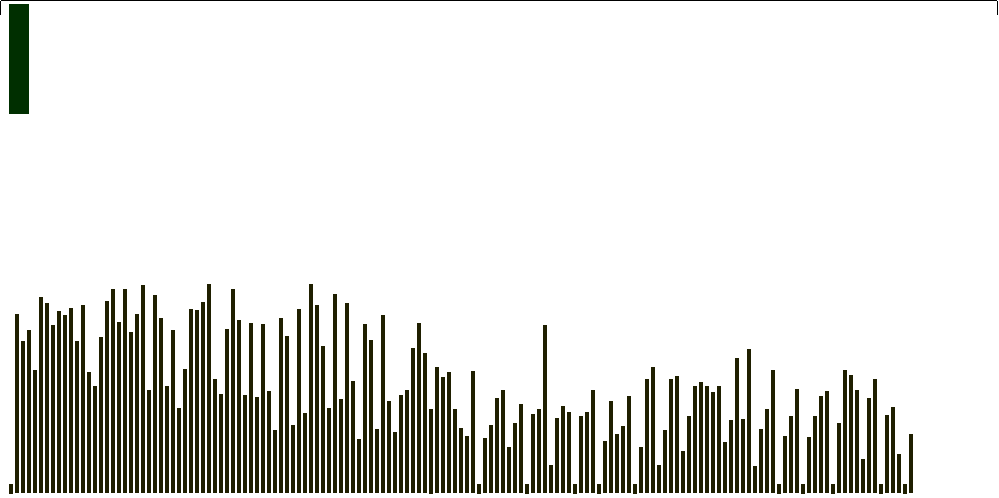
\includegraphics[scale=0.5]{pic5000_h.png}
        \paragraph{}
            低位哈希时,20000条记录在所有桶上的分布情况
        \paragraph{}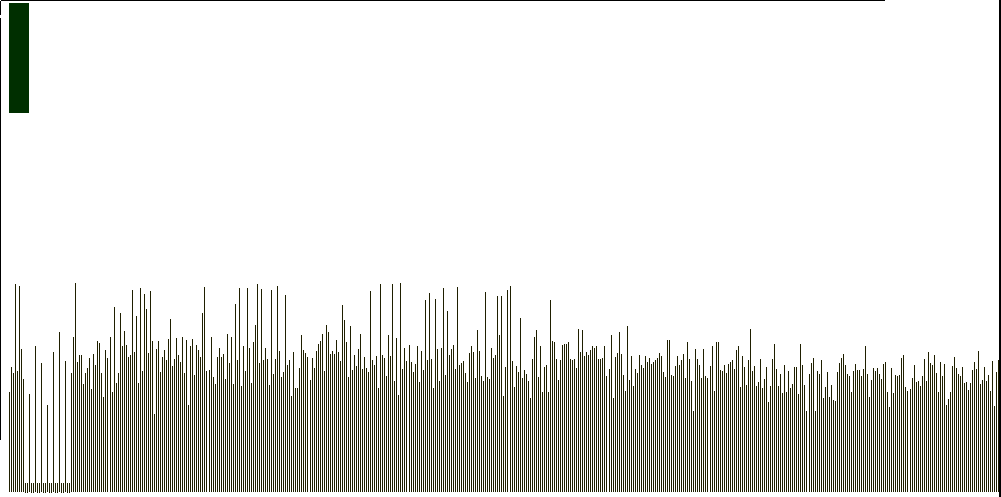
\includegraphics[scale=0.5]{pic20000_l.png}
        \paragraph{}
            高位哈希时,20000条记录在所有桶上的分布情况
        \paragraph{}
\includegraphics[scale=0.5]{pic20000_h.png}
    \subsection{IO次数}
        \paragraph{}
            为了省时起见,我们用脚本截取了20万条记录进行测试,对于同样的数据四种版本的对比如下:
        \begin{itemize}
            \item 8页,低位哈系,107857次
            \item 8页,高位哈系,67844次
            \item 128页,高位哈系,12227次
            \item 128页,低位哈系,99591次
        \end{itemize}
        \paragraph{}
            可见高位哈希由于一开始初始化好了目录,在IO上对低位有优势。
\section{总结}
    \begin{itemize}
        \item 由纯C写成,调试经常因为野指针的问题时困难重重。后期又重写了一个python的原型进行测试,由此修复不少问题。
        \item 由于疲劳很容易犯各种错误,一旦出现非常难找到。工程代码很需要头脑清醒。
        \item 写出来的代码类似于操作系统做的事情,比如换页、IO请求等,加深了对数据库系统和系统这个概念的理解。
    \end{itemize}
\end{document}
